\section{\Acrfull{bsj} detection}

For detection of \glspl{bsj}, I used the five tools already introduced in
\cref{subsec:circrna_detection}.
As shown in \cref{fig:detection_bars}, find\_circ, CIRI2, DCC, and
circexplorer2 detect a similar number of \glspl{bsj}, while segemehl detects
almost ten times as many \glspl{bsj} as its closest competitor, DCC.

\begin{figure}[H] \centering

    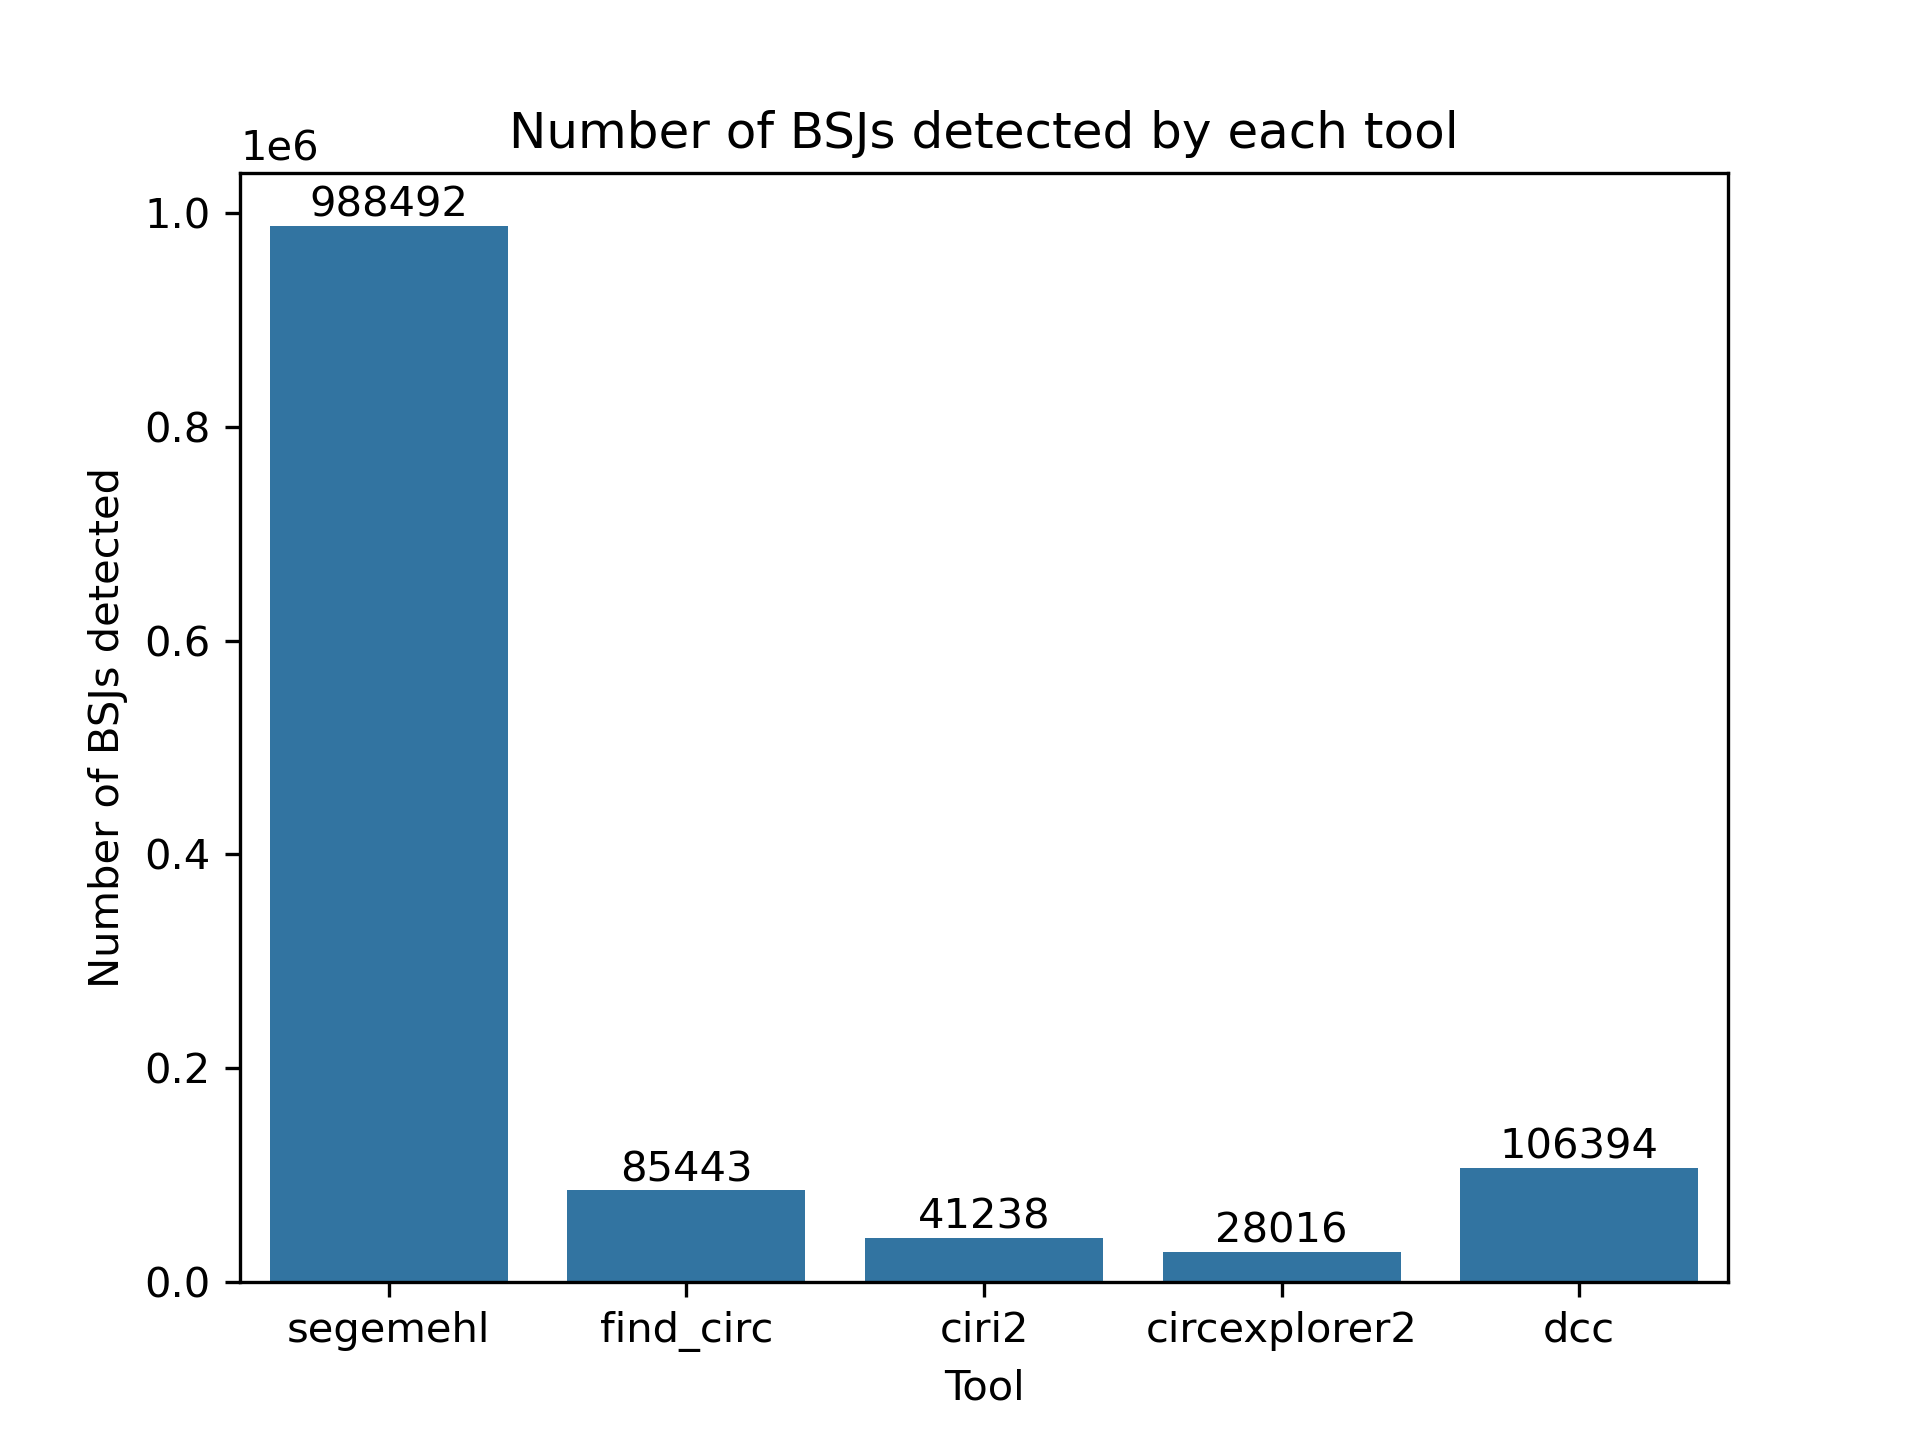
\includegraphics[width=0.6\textwidth]{chapters/4_results_and_discussion/figures/detection/n_bsjs_detected.png}
    \caption{Number of \glspl{bsj} detected by each tool.
        While find\_circ, CIRI2, DCC and circexplorer2 detect a similar number of
        \glspl{bsj}, segemehl detects a much larger number of \glspl{bsj}.
    }
    \label{fig:detection_bars}
\end{figure}
Similar behavior was previously observed by \textcite{zeng_comprehensive_2017},
where segemehl was among the top performers in terms of sensitivity, but also
had a high false positive rate.
The lowest numbers of \glspl{bsj} were detected by circexplorer2 and CIRI2,
which both have built-in filters to reduce false
positives\supercite{zhang_diverse_2016,gao_circular_2018}.

\subsection{Agreement between tools}

Although tools like CIRI2 and CircExplorer2 have shown good performance in
benchmarks\supercite{zeng_comprehensive_2017}, having multiple tools agree on
the same \gls{bsj} leads to even better robustness of the
detection\supercite{hansen_comparison_2016}.

To assess the agreement between the tools, I used UpSet plots, which show the
overlap of \glspl{bsj} detected by different tools.
When identifying the overlap between tools, the most strict approach is to
consider only \glspl{bsj} with identical start and end positions and on the
same strand as the same \gls{bsj}.
The according plot is shown in \cref{fig:detection_upset_0_stranded}.

\begin{figure}[H]
    \centering

    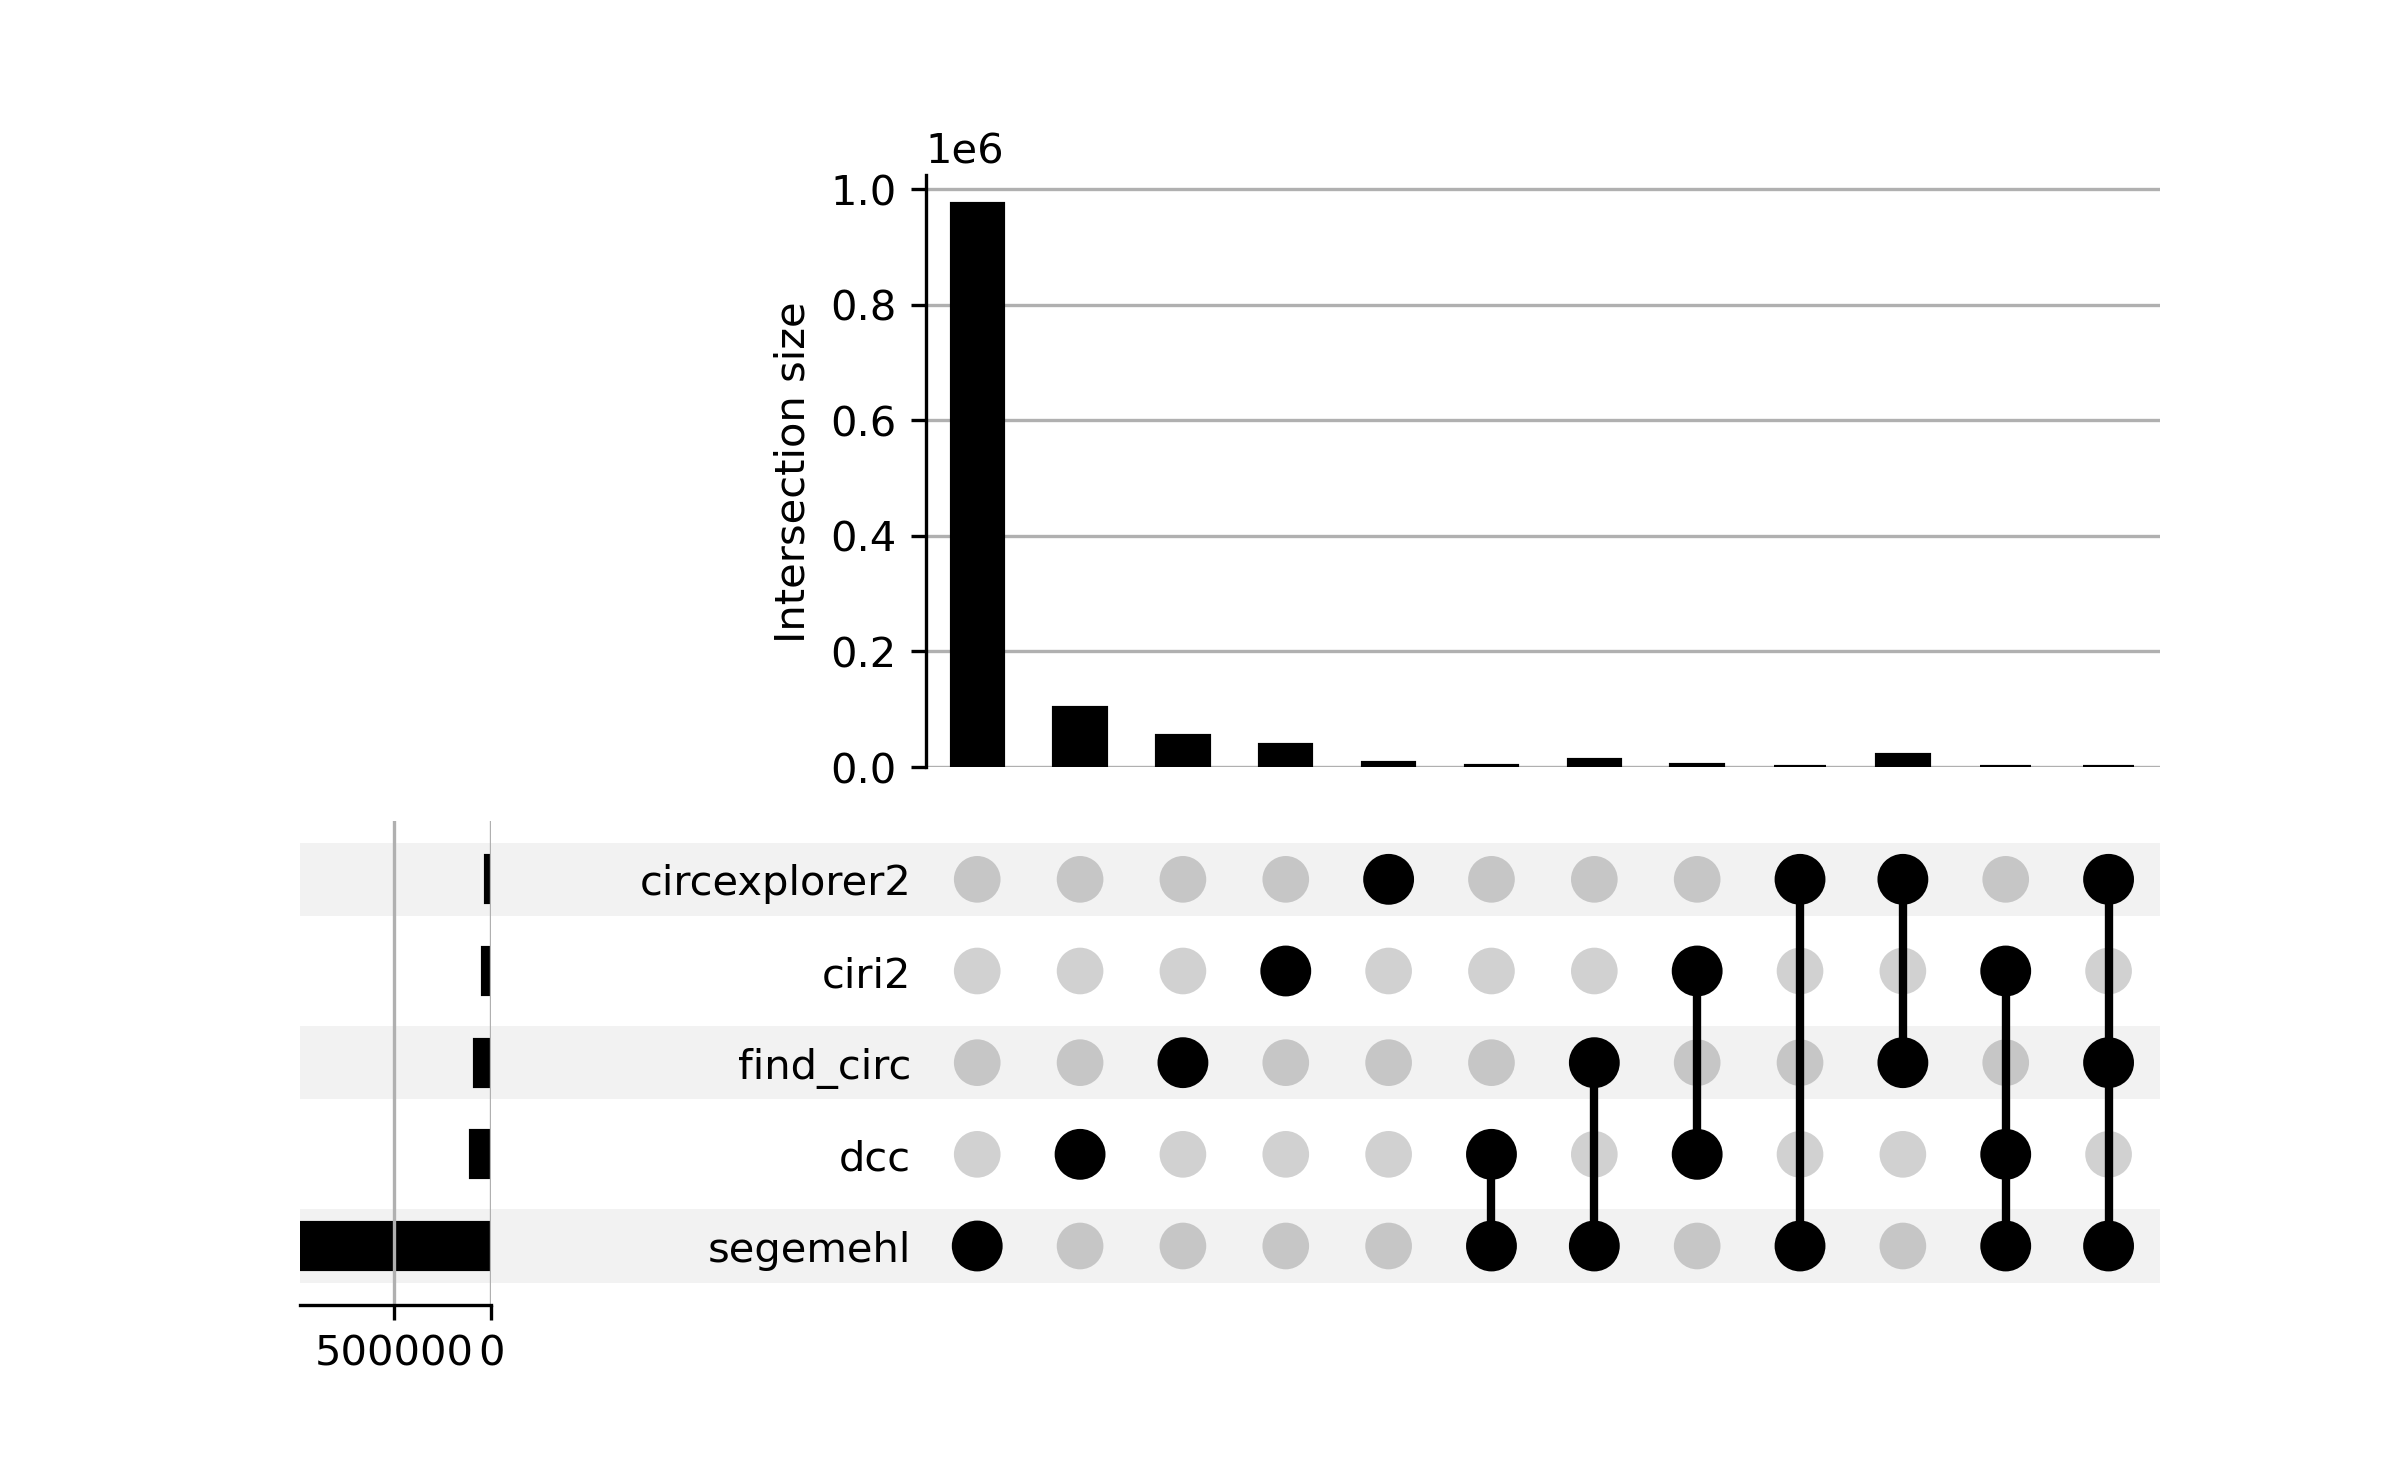
\includegraphics[width=\textwidth]{chapters/4_results_and_discussion/figures/detection/upset/shift_0_stranded.png}
    \caption{Upset plot illustrating the overlap between \glspl{bsj} detected
        by different tools.
        Only \glspl{bsj} with identical start and end positions on the same strand are
        considered the same.
    } \label{fig:detection_upset_0_stranded} \end{figure}

As this agreement is relatively low, I investigated the detected \glspl{bsj}
more closely and found that across tools and samples, in many cases
\glspl{crna} are detected with very small differences in the start and end
positions, or on different strands.
When applying the strict matching criteria of identical start and end positions
on the same strand, many \glspl{bsj} are not considered to be the same, even
though they likely represent the same \gls{crna}.
In the following sections, I will investigate the role of the \textit{max
    shift} parameter and strandedness in the agreement between tools.

\subsubsection{The role of the \textit{max shift} parameter}

In order to quantify how frequently slight shifts in start and end positions
between \glspl{bsj} occur, I introduced a \textit{max shift} parameter.
With this parameter, a pair of \glspl{bsj} is considered to be the same if both
the start and end positions differ by at most \textit{max shift} nucleotides.
A more detailed explanation is given in \cref{fig:detection_shift_schematic}.

\begin{figure}[H] \centering

    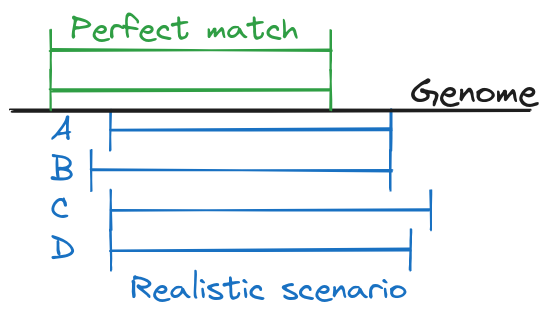
\includegraphics[width=0.7\textwidth]{chapters/4_results_and_discussion/figures/grouping.png}
    \caption{Schematic illustrating two different scenarios of \gls{bsj}
        matches across tools.
        In the \textit{perfect match} scenario, the \glspl{bsj} are exactly the same.
        This is what is required in order to be counted as a match in
        \cref{fig:detection_upset_0_stranded}.
        However, this rarely occurs in the data used in this study.
        More frequently, the \textit{realistic scenario} occurs.
        Here, very similar \glspl{bsj} are detected, with only a few nucleotides
        difference.
        In order to account for this, a \textit{max shift} parameter is introduced.
        While with the \textit{perfect match} approach, there would not be any matches
        between \glspl{bsj} at all, with a \textit{max shift} of 1, the result would
        change drastically.
        The \gls{bsj} marked as A would match with two others (B and D), similarly B
        would match with A and D.
        C would only match with D, as both the ends of both A and B differ by more than
        1.
        D would match with all others.
        A \textit{max shift} of 2 would lead to matches between all \glspl{bsj}.
    }
    \label{fig:detection_shift_schematic}
\end{figure}

In order to quantify the magnitude of the effect of the \textit{max shift}
parameter, I calculated the level of agreement between tools for different
values of \textit{max shift}.
The results are shown in \cref{fig:shift_agreement_stranded}.

\begin{figure}[H]
    \centering

    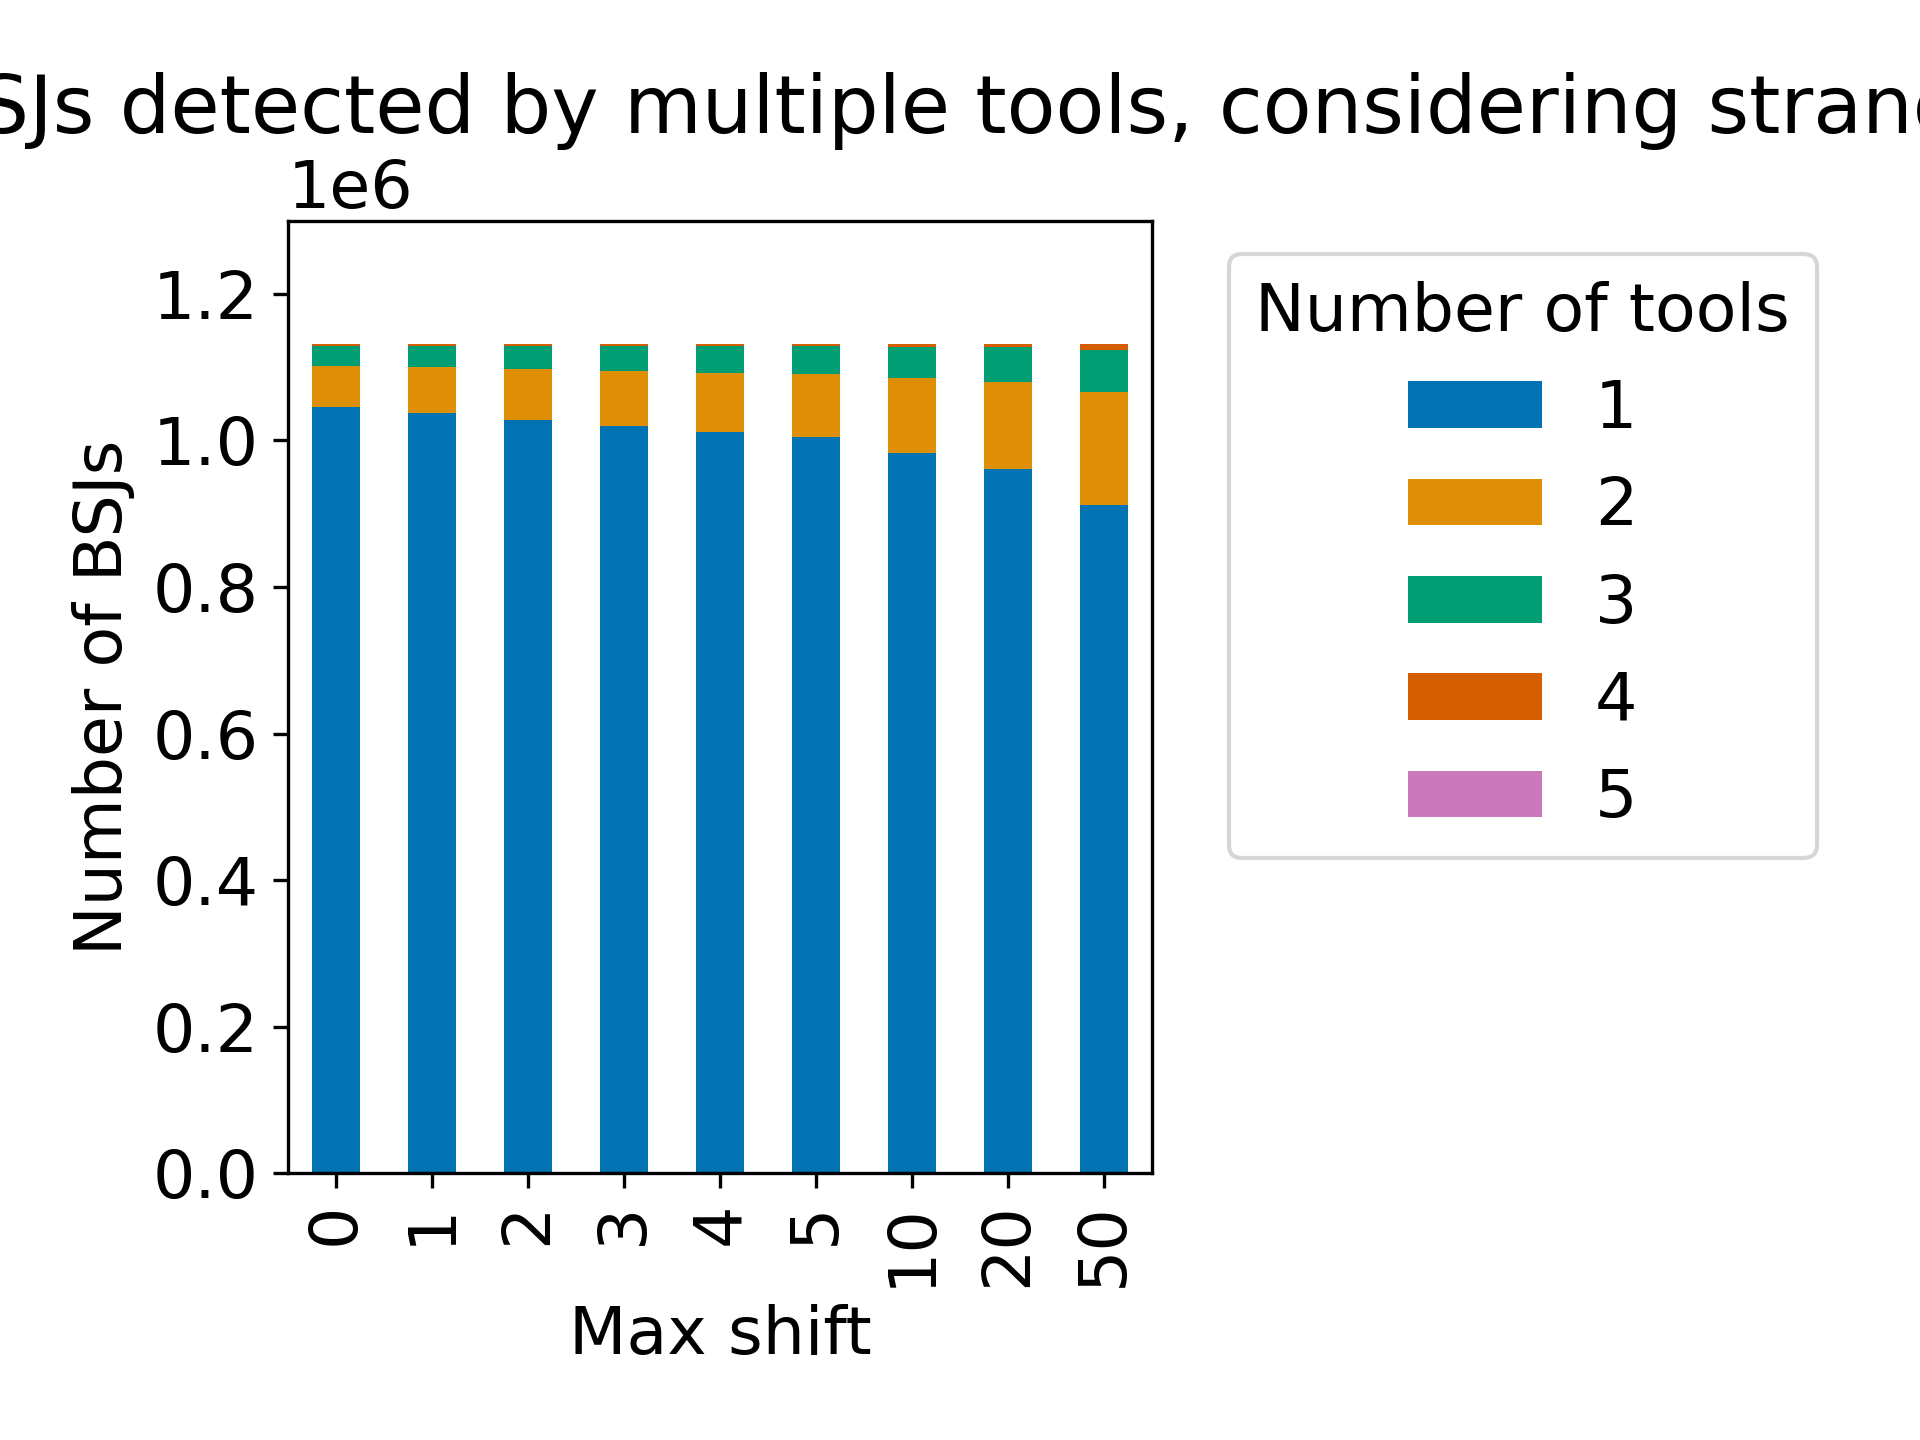
\includegraphics[width=0.7\textwidth]{chapters/4_results_and_discussion/figures/detection/shift_agreement_stranded.png}
    \caption{Stacked bar plot showing the level of agreement between tools for
        different values of the \textit{max shift} parameter.
        Strand information is considered.
    }
    \label{fig:shift_agreement_stranded}
\end{figure}

As shown in \cref{fig:shift_agreement_stranded}, the distribution of the number
of tools supporting a \gls{bsj} changes drastically when increasing the
\textit{max shift} parameter from 0 to 1.
In contrast, increasing the \textit{max shift} parameter to higher values has
only a minor effect on the distribution.
While the number of \glspl{bsj} detected by 2 tools keeps increasing, the
number of \glspl{bsj} detected by more than two tools remains relatively
stable.
While with low values of the \textit{max shift} parameter, one can be
relatively sure that the matched hits actually represent the same \gls{crna},
increasing the \textit{max shift} parameter to large values comes with the risk
of overlooking biological differences.
I am not aware of a study that has systematically investigated the effect of
such shifts on the detection of \glspl{bsj}.
Also, due to the lack of a ground truth, it is impossible to determine the
optimal value for the \textit{max shift} parameter.

\subsubsection{The role of strandedness}

In order to investigate the effect of strandedness on the agreement between
tools, I repeated the analysis, this time also allowing matches between
\glspl{bsj} on different strands.

\begin{figure}[H]
    \centering

    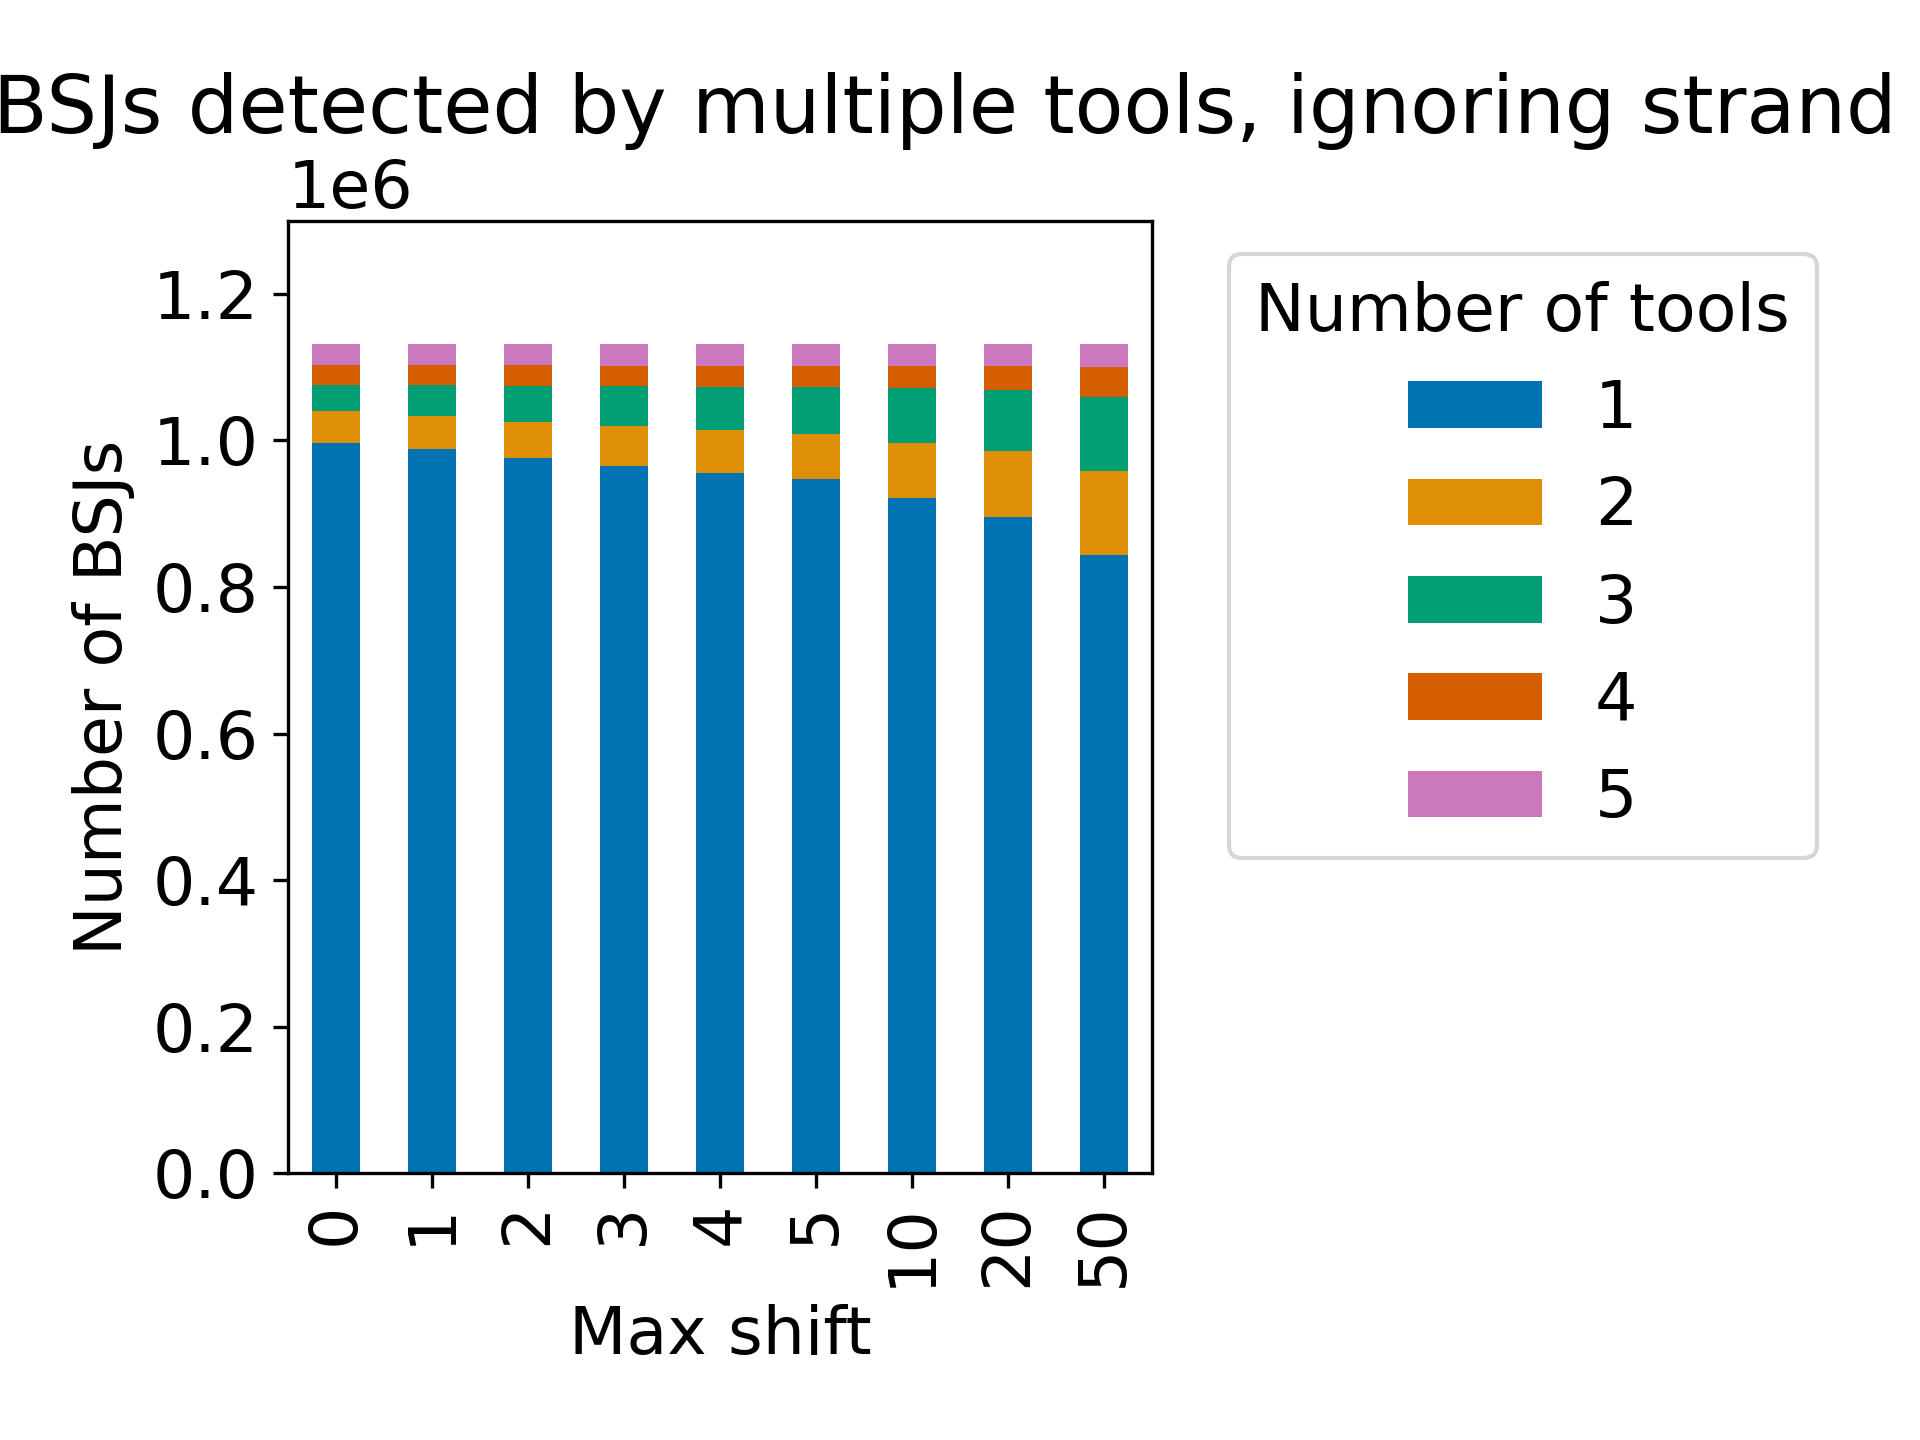
\includegraphics[width=0.7\textwidth]{chapters/4_results_and_discussion/figures/detection/shift_agreement_unstranded.png}
    \caption{Stacked bar plot showing the level of agreement between tools for
        different values of the \textit{max shift} parameter.
        Strand information is ignored.
    }
    \label{fig:shift_agreement_unstranded}
\end{figure}

Strikingly, the agreement between tools is much higher when ignoring
strandedness.
When using a \textit{max shift} parameter of 0, the number of \glspl{bsj}
detected by two or more tools is increases from x to y.
When increasing the \textit{max shift} parameter to 1, a substantial number of
\glspl{bsj} are detected by four and even all five tools.
This is in stark contrast to the results when considering strandedness, where
the number of \glspl{bsj} detected by four or five tools is very low, even with
large values of the \textit{max shift} parameter.
This suggests that there might be a technical or biological issue in the strand
information.
Investigating this further is beyond the scope of this thesis, but might be an
interesting topic for future research.

\subsubsection{Selecting thresholds}

For the following analyses, I chose a \textit{max shift} parameter of 3 and a
minimum agreement of 4 tools, as this appeared to be a good compromise between
sensitivity and specificity.
Strand information was ignored.
The resulting UpSet plot is shown in \cref{fig:detection_upset_3_nostrand}.

\begin{figure}[H]
    \centering

    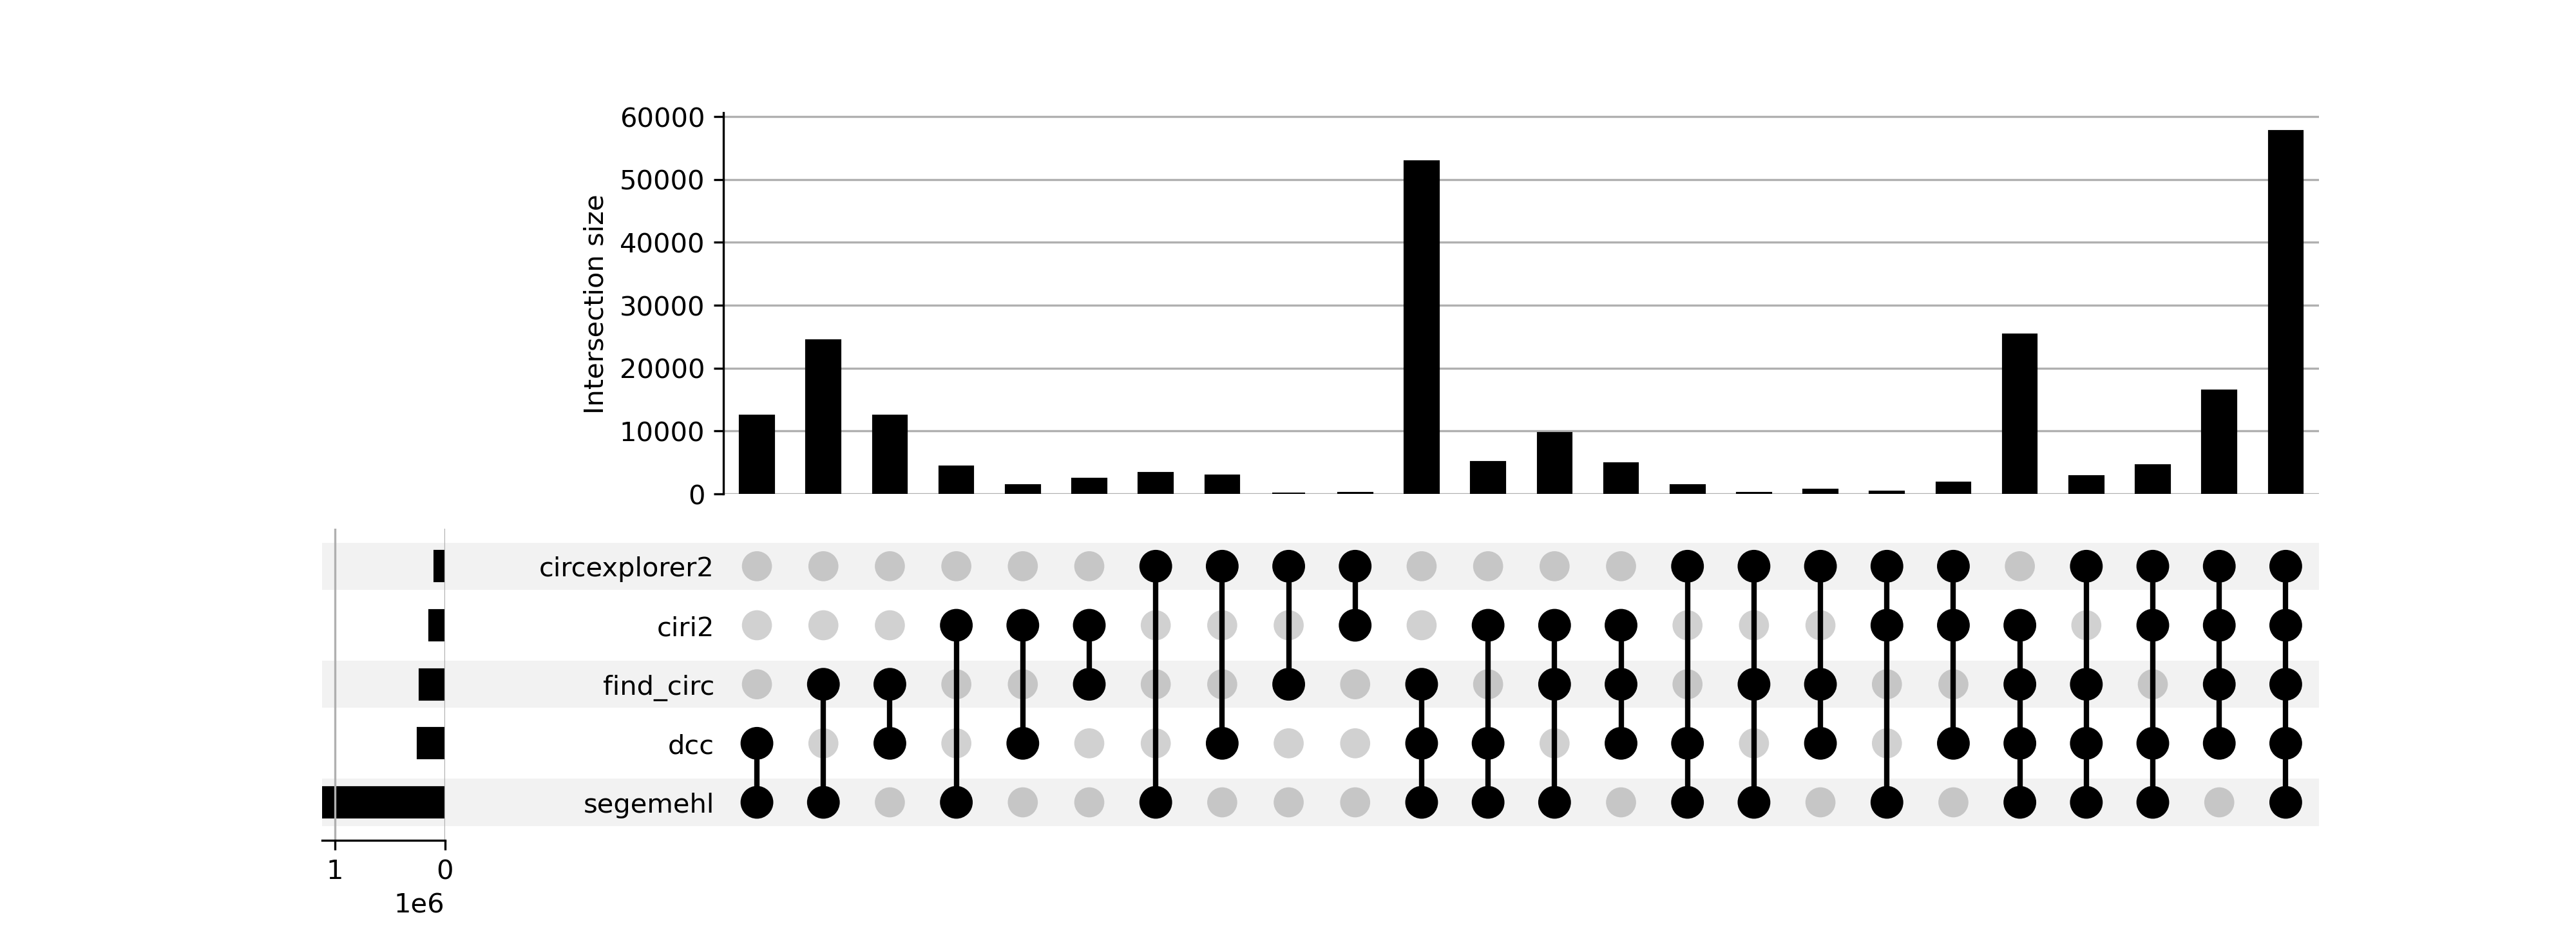
\includegraphics[width=\textwidth]{chapters/4_results_and_discussion/figures/detection/upset/shift_3_unstranded.png}
    \caption{Upset plot illustrating the overlap between \glspl{bsj} detected
        by
        different tools.
        Agreement was calculated using a \textit{max shift} of 3 and ignoring strand
        information.
        Only combinations including at least 2 tools and 10 common \glspl{bsj} are
        shown.
    }
    \label{fig:detection_upset_3_nostrand}
\end{figure}

\subsection{circRNA types}

\begin{figure}[H]
    \centering

    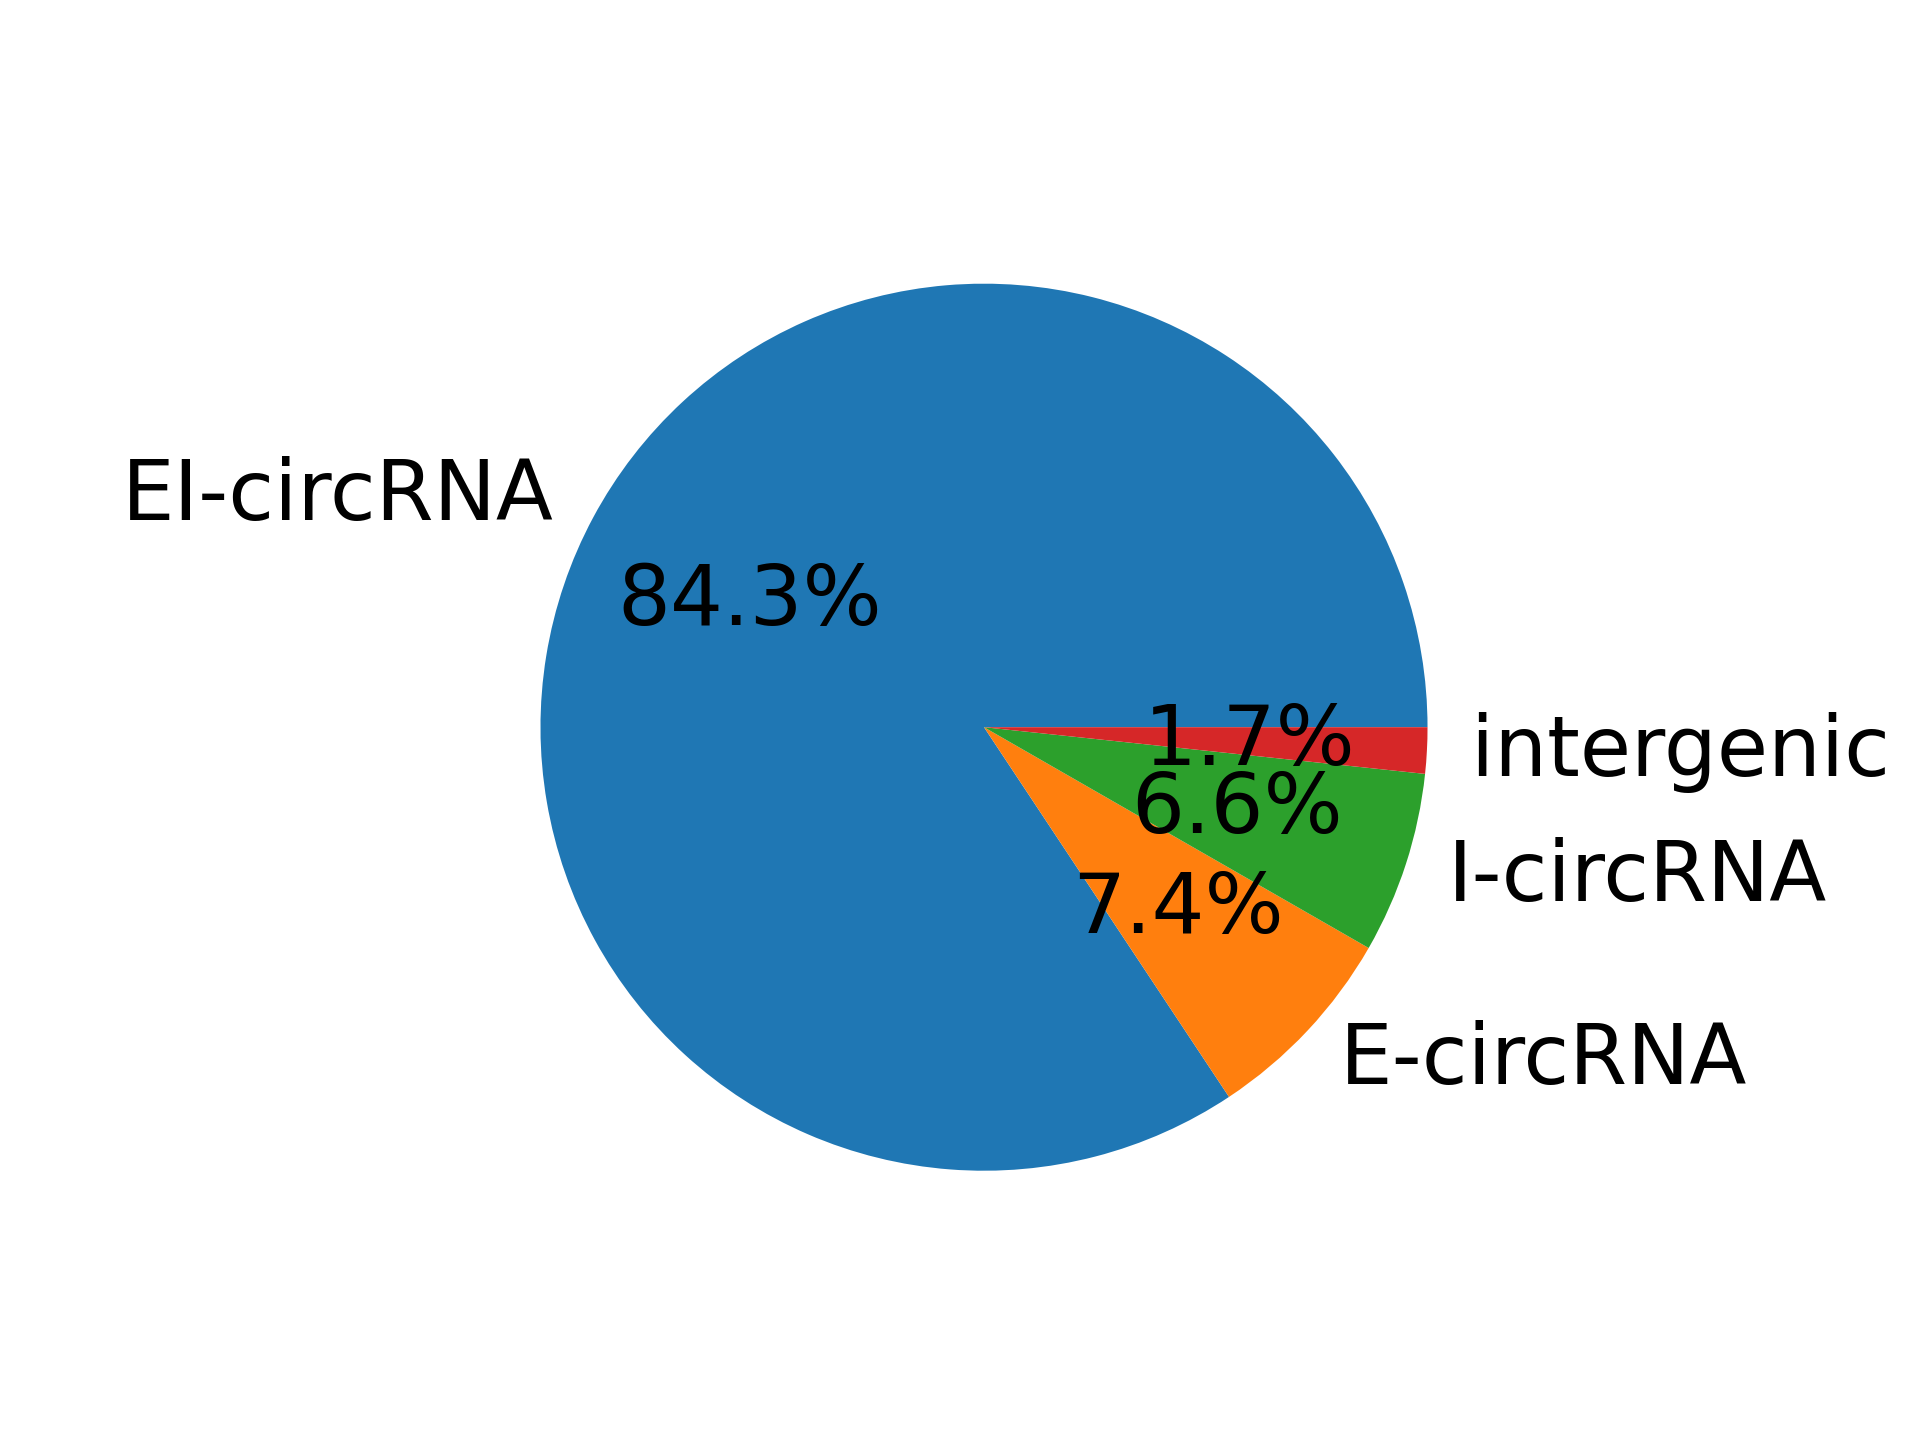
\includegraphics[width=0.5\textwidth]{chapters/4_results_and_discussion/figures/detection/types.png}
    \caption{Pie chart showing the distribution of different types of
        \glspl{crna} detected by the pipeline.
        While according to literature \glspl{e-crna} are the most abundant type of
        \glspl{crna}, here we see \glspl{ei-crna} as the most abundant type.
        This is most likely due to the fact that we only know the start and end
        positions of the \glspl{bsj}, but not the internal structure of the
        \glspl{crna}.
        Thus, \glspl{crna} are only labeled as \glspl{e-crna} if they are fully
        contained in a single exon.
        If they span multiple exons (thus, overlapping with at least one intron), they
        are labeled as \glspl{ei-crna}.
    }
    \label{fig:circrna_types}
\end{figure}

\subsection{Database agreement}
\begin{figure}[ht] \begin{tabular}{cc}
        \begin{subfigure}{0.5\textwidth} \centering

            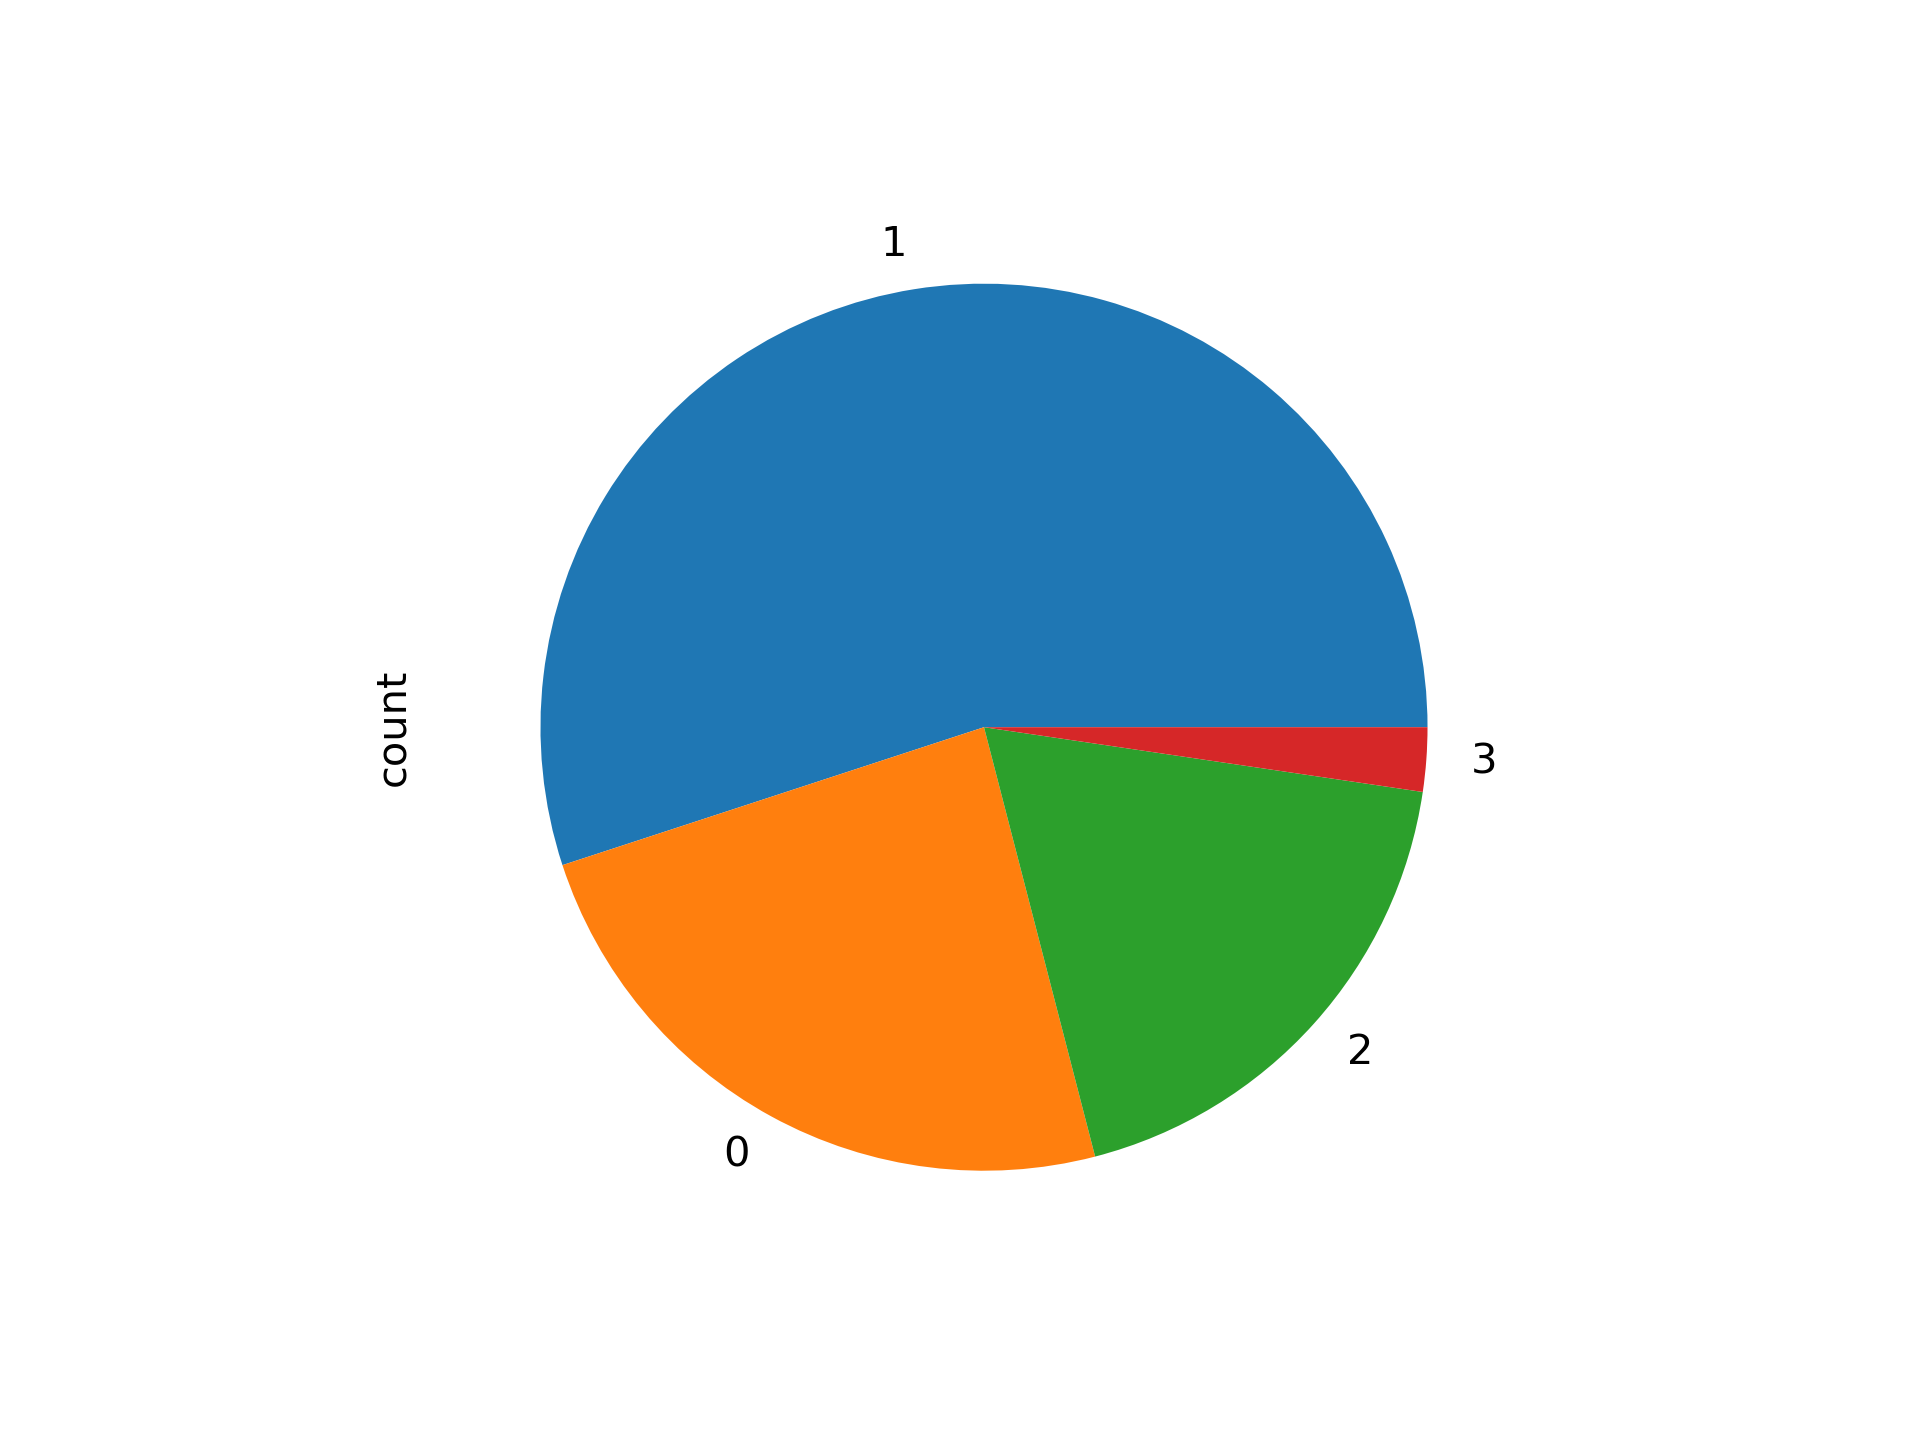
\includegraphics[width=\linewidth]{chapters/4_results_and_discussion/figures/detection/database_count.png}
            \caption{Fractions of \glspl{crna} supported by
                different numbers of databases}
            \label{fig:db_pie}
        \end{subfigure}
        \begin{subfigure}{0.5\textwidth}
            \centering

            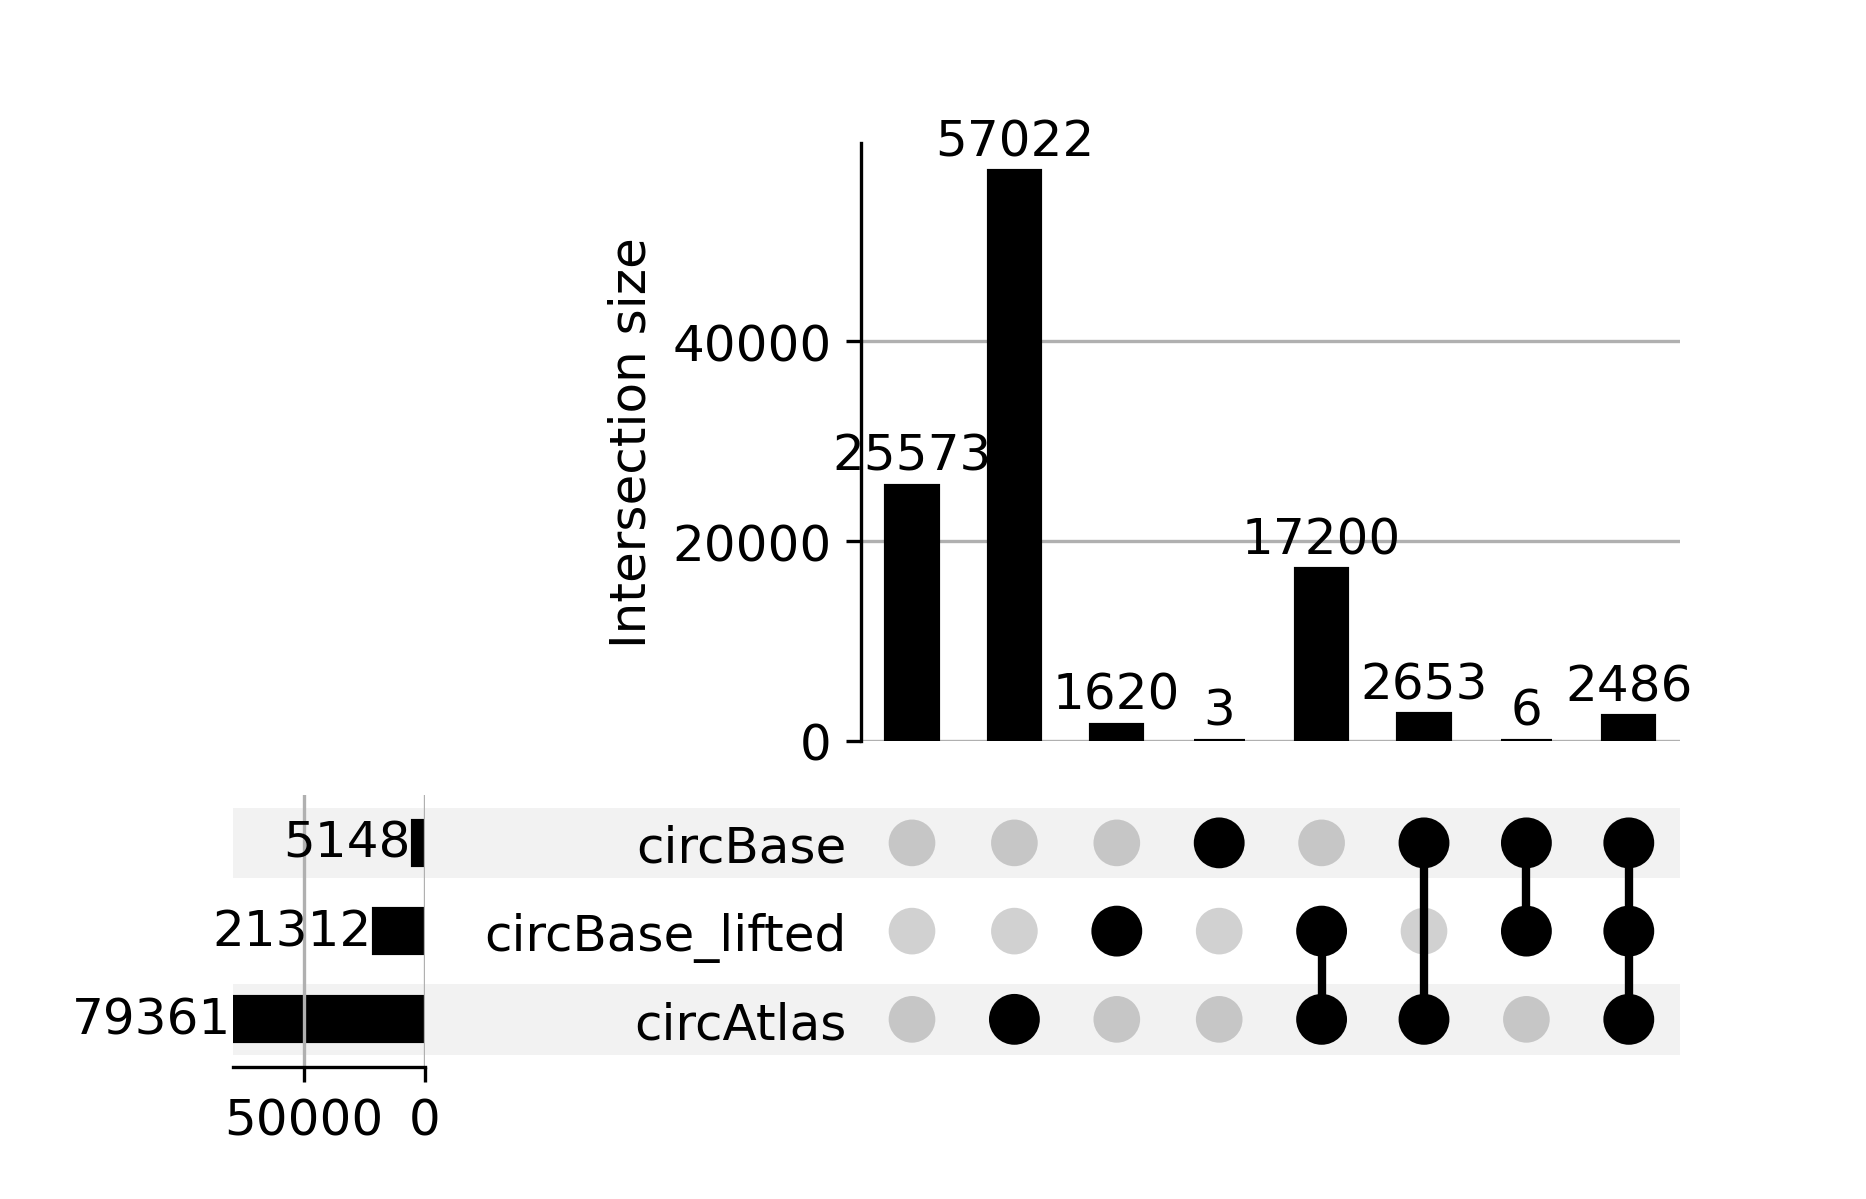
\includegraphics[width=\linewidth]{chapters/4_results_and_discussion/figures/detection/database_upset.png}
            \caption{Agreement between detected
                \glspl{bsj} and databases}
            \label{fig:db_upset}
        \end{subfigure} &

    \end{tabular}
    \caption{As \cref{fig:db_pie} shows, while there is a large fraction of
        \glspl{crna} without any
        database match, more than 50\% of detected \glspl{crna} at least one
        hit.
        As shown in \cref{fig:db_upset}, most hits are from circAtlas, which is most
        likely due to the fact that it is the largest database.
        While both circBase and circBase\_lifted have some exclusive hits, the majority
        of their hits are shared with circAtlas.
    }
    \label{fig:db_agreement}
\end{figure}
